\documentclass[12pt,a4paper]{article}
\usepackage{fontspec}
\setmainfont{FreeSerif}
\setsansfont{FreeSans}
\setmonofont{FreeMono}[Scale=0.9]
\usepackage[a4paper,margin=2.5cm]{geometry}
\usepackage{graphicx}
\graphicspath{{../figures/}}
\usepackage{booktabs,float,array,xcolor,amsmath,enumitem,subcaption,caption}
\usepackage{tikz}
\usetikzlibrary{arrows.meta,positioning,shapes.geometric,fit,backgrounds}
\usepackage{listings}
\usepackage[colorlinks=true,linkcolor=blue!50!black,urlcolor=blue!50!black]{hyperref}
\lstset{basicstyle=\ttfamily\footnotesize,breaklines=true,frame=single,backgroundcolor=\color{gray!8},columns=fullflexible,keepspaces=true}
\setlength{\parskip}{4pt}\sloppy
\renewcommand{\arraystretch}{1.12}
\renewcommand{\contentsname}{Mục lục}
\renewcommand{\figurename}{Hình}
\renewcommand{\tablename}{Bảng}
\newcommand{\TabData}{%
\begin{table}[H]\centering\small\setlength{\tabcolsep}{6pt}
\caption{Thống kê bộ dữ liệu trước và sau khi loại tin nhắn trùng lặp.}\label{tab:data}
\begin{tabular}{lrrrr}\toprule
Tập & Tổng & Ham & Spam & Tỉ lệ spam \\\midrule
Dữ liệu thô & 5574 & 4827 & 747 & 13,4\% \\
Sau khi bỏ trùng & 5171 & 4518 & 653 & 12,6\% \\
Train (80\%) & 4136 & 3614 & 522 & 12,6\% \\
Test (20\%) & 1035 & 904 & 131 & 12,7\% \\\bottomrule
\end{tabular}\end{table}}

\newcommand{\TabSignal}{%
\begin{table}[H]\centering\small\setlength{\tabcolsep}{6pt}
\caption{Đặc điểm khác biệt giữa ham và spam (sau khi bỏ trùng).}\label{tab:signal}
\begin{tabular}{lrr}\toprule
Đặc điểm & Ham & Spam \\\midrule
Độ dài trung bình (ký tự) & 70,9 & 137,7 \\
Độ dài trung vị (ký tự) & 53 & 148 \\
Độ dài lớn nhất (ký tự) & 910 & 223 \\
Số từ trung bình & 14,2 & 23,7 \\
Chứa chuỗi $\geq 5$ chữ số & 0,1\% & 76,7\% \\
Chứa URL/tên miền & 0,3\% & 17,8\% \\
Chứa ký hiệu tiền tệ & 0,4\% & 33,2\% \\
Tỉ lệ chữ HOA trung bình & 7,7\% & 16,6\% \\\bottomrule
\end{tabular}\end{table}}

\newcommand{\TabCfg}{%
\begin{table}[H]\centering\scriptsize\setlength{\tabcolsep}{3pt}
\caption{Cấu hình được chọn cho từng mô hình (chọn theo F1 của 5-fold CV trên tập train).}\label{tab:cfg}
\begin{tabular}{lllp{3.4cm}rr}\toprule
Mô hình & Tiền xử lý & Biểu diễn & Siêu tham số & CV-F1 mặc định & CV-F1 tinh chỉnh \\\midrule
Multinomial NB & P2\_norm\_stop & BoW\_uni & alpha=2,0, fit\_prior=True & 0,9400 & 0,9518 \\
K-NN & P1\_normalize & TFIDF\_uni & metric=cosine, n\_neighbors=9, weights=distance & 0,8759 & 0,9176 \\
Cây quyết định & P2\_norm\_stop & BoW\_uni & criterion=gini, max\_depth=10, min\_samples\_leaf=1 & 0,9072 & 0,9110 \\\bottomrule
\end{tabular}\end{table}}

\newcommand{\TabBaseTuned}{%
\begin{table}[H]\centering\small\setlength{\tabcolsep}{6pt}
\caption{Kết quả trên tập test: baseline (BoW unigram, không tiền xử lý, tham số mặc định) và cấu hình tinh chỉnh. Spam là lớp dương.}\label{tab:basetuned}
\begin{tabular}{llrrrr}\toprule
Mô hình & Phương án & Accuracy & Precision & Recall & F1 \\\midrule
Multinomial NB & Baseline & 0,9807 & 0,9512 & 0,8931 & 0,9213 \\
 & Tinh chỉnh & 0,9913 & 0,9766 & 0,9542 & \textbf{0,9653} \\
K-NN & Baseline & 0,9072 & 1,0000 & 0,2672 & 0,4217 \\
 & Tinh chỉnh & 0,9826 & 0,9593 & 0,9008 & \textbf{0,9291} \\
Cây quyết định & Baseline & 0,9691 & 0,9024 & 0,8473 & 0,8740 \\
 & Tinh chỉnh & 0,9874 & 1,0000 & 0,9008 & \textbf{0,9478} \\\bottomrule
\end{tabular}\end{table}}

\newcommand{\TabFinal}{%
\begin{table}[H]\centering\small\setlength{\tabcolsep}{6pt}
\caption{Kết quả cuối cùng trên tập test (1035 tin nhắn, 131 spam), một lần chia với random\_state=42.}\label{tab:final}
\begin{tabular}{lrrrrrr}\toprule
Mô hình & Accuracy & Precision & Recall & F1 & ROC-AUC & FP / FN \\\midrule
Multinomial NB & 0,9913 & 0,9766 & 0,9542 & 0,9653 & 0,9860 & 3 / 6 \\
K-NN & 0,9826 & 0,9593 & 0,9008 & 0,9291 & 0,9919 & 5 / 13 \\
Cây quyết định & 0,9874 & 1,0000 & 0,9008 & 0,9478 & 0,9500 & 0 / 13 \\\bottomrule
\end{tabular}\end{table}}

\newcommand{\TabSeeds}{%
\begin{table}[H]\centering\scriptsize\setlength{\tabcolsep}{3pt}
\caption{Độ ổn định: trung bình $\pm$ độ lệch chuẩn trên 5 lần chia train/test khác nhau (seed 0--4), siêu tham số giữ cố định.}\label{tab:seeds}
\begin{tabular}{lccccc}\toprule
Mô hình & Accuracy & Precision & Recall & F1 & ROC-AUC \\\midrule
Multinomial NB & 0,9865 $\pm$ 0,0050 & 0,9470 $\pm$ 0,0280 & 0,9466 $\pm$ 0,0179 & 0,9467 $\pm$ 0,0195 & 0,9879 $\pm$ 0,0053 \\
K-NN & 0,9838 $\pm$ 0,0032 & 0,9662 $\pm$ 0,0129 & 0,9038 $\pm$ 0,0368 & 0,9335 $\pm$ 0,0147 & 0,9809 $\pm$ 0,0045 \\
Cây quyết định & 0,9778 $\pm$ 0,0040 & 0,9611 $\pm$ 0,0214 & 0,8595 $\pm$ 0,0257 & 0,9073 $\pm$ 0,0175 & 0,9450 $\pm$ 0,0146 \\\bottomrule
\end{tabular}\end{table}}

\newcommand{\TabAlpha}{%
\begin{table}[H]\centering\small\setlength{\tabcolsep}{6pt}
\caption{Độ nhạy của Multinomial NB theo $\alpha$ (CV-F1 trung bình qua 3 cách chia fold; cấu hình P2 + BoW unigram).}\label{tab:alpha}
\begin{tabular}{rrrr}\toprule
$\alpha$ & F1 & Precision & Recall \\\midrule
0,1 & 0,9396 & 0,9314 & 0,9483 \\
0,5 & 0,9390 & 0,9278 & 0,9508 \\
1 & 0,9396 & 0,9315 & 0,9483 \\
2 & 0,9503 & 0,9541 & 0,9470 \\
3 & 0,9488 & 0,9622 & 0,9361 \\
5 & 0,9460 & 0,9725 & 0,9214 \\
10 & 0,9409 & 0,9826 & 0,9029 \\\bottomrule
\end{tabular}\end{table}}

\newcommand{\TabVecGrid}{%
\begin{table}[H]\centering\small\setlength{\tabcolsep}{6pt}
\caption{F1 CV (5-fold, tập train) theo n-gram và \texttt{min\_df}, các tham số khác giữ nguyên (\texttt{max\_df}=1,0). Với \texttt{max\_df}=0,5 cho kết quả \emph{giống hệt}.}\label{tab:vecgrid}
\begin{tabular}{llrrrr}\toprule
Mô hình & Biểu diễn & min\_df=1 & 2 & 3 & 5 \\\midrule
Multinomial NB & unigram & 0,9518 & 0,9412 & 0,9407 & 0,9357 \\
 & unigram + bigram & 0,9492 & 0,9443 & 0,9432 & 0,9408 \\
K-NN & unigram & 0,9176 & 0,9213 & 0,9219 & 0,9188 \\
 & unigram + bigram & 0,9112 & 0,9130 & 0,9201 & 0,9218 \\
Cây quyết định & unigram & 0,9110 & 0,9020 & 0,9106 & 0,9125 \\
 & unigram + bigram & 0,8985 & 0,9034 & 0,8952 & 0,8944 \\\bottomrule
\end{tabular}\end{table}}

\newcommand{\TabVecFeat}{%
\begin{table}[H]\centering\small\setlength{\tabcolsep}{6pt}
\caption{F1 CV theo số đặc trưng tối đa (\texttt{max\_features}, unigram); cột cuối là toàn bộ từ vựng (khoảng 6\,500 từ).}\label{tab:vecfeat}
\begin{tabular}{lrrrrrr}\toprule
Mô hình & 200 & 500 & 1000 & 2000 & 5000 & Tất cả \\\midrule
Multinomial NB & 0,9116 & 0,9332 & 0,9356 & 0,9433 & 0,9499 & 0,9518 \\
K-NN & 0,9041 & 0,9164 & 0,9187 & 0,9229 & 0,9188 & 0,9176 \\
Cây quyết định & 0,9015 & 0,9089 & 0,9123 & 0,9089 & 0,9037 & 0,9110 \\\bottomrule
\end{tabular}\end{table}}

\newcommand{\NBtopspam}{\texttt{longnumtoken}, \texttt{claim}, \texttt{prize}, \texttt{nokia}, \texttt{tone}, \texttt{guaranteed}, \texttt{ppm}, \texttt{cs}, \texttt{awarded}, \texttt{ringtone}}

\newcommand{\NBtopham}{\texttt{gt}, \texttt{lt}, \texttt{lor}, \texttt{home}, \texttt{come}, \texttt{later}, \texttt{da}, \texttt{ok}, \texttt{really}, \texttt{going}}

\newcommand{\DTtop}{\texttt{longnumtoken} (0.746), \texttt{urltoken} (0.076), \texttt{numtoken} (0.038), \texttt{reply} (0.019), \texttt{mobile} (0.016), \texttt{currtoken} (0.009)}


\newcommand{\spam}{\textit{spam}}
\newcommand{\ham}{\textit{ham}}

\begin{document}

\begin{titlepage}
\centering
{\large TRƯỜNG ĐẠI HỌC ĐẠI NAM --- KHOA CÔNG NGHỆ THÔNG TIN}\\[1.2cm]
{\Large \textbf{BÁO CÁO BÀI TẬP LỚN}}\\[0.3cm]
{\large Học phần: Nhập môn Học máy (FIT4013)}\\[1.8cm]
{\LARGE \textbf{ĐỀ TÀI 3: PHÂN LOẠI TIN NHẮN RÁC}}\\[0.4cm]
{\large SMS Spam Collection --- Multinomial Naive Bayes, K-NN và Cây quyết định}\\[2cm]
\begin{tabular}{ll}
Giảng viên hướng dẫn: & ThS. Lê Thị Thùy Trang\\
Nhóm thực hiện: & \textbf{[Số nhóm]}\\
Thành viên: & \textbf{[Họ tên -- MSSV -- vai trò]}\\
 & \textbf{[Họ tên -- MSSV -- vai trò]}\\
Repository: & \textbf{[Liên kết GitHub của nhóm]}\\
\end{tabular}
\vfill
{\large Năm học 2026--2027}
\end{titlepage}

\tableofcontents
\newpage

% ====================================================================
\section{Đặt vấn đề và phân tích yêu cầu}
\subsection{Bối cảnh và mục tiêu}
Tin nhắn rác (SMS spam) gây phiền toái, tốn chi phí và là kênh phổ biến của lừa đảo. Bài toán là xây dựng bộ phân loại tự động cho biết một tin nhắn văn bản là \spam{} (tin rác) hay \ham{} (tin hợp lệ). Đây là bài toán \textbf{phân loại nhị phân học có giám sát} trên dữ liệu văn bản, với lớp \spam{} được xem là lớp dương.

Mục tiêu của nhóm: (i) khảo sát dữ liệu; (ii) so sánh các cách tiền xử lý và biểu diễn văn bản (Bag-of-Words, TF-IDF, unigram/bigram); (iii) huấn luyện và so sánh ba thuật toán đã học là Multinomial Naive Bayes, K-NN và Cây quyết định so với một baseline; (iv) đánh giá bằng nhiều độ đo thay vì chỉ Accuracy và phân tích các trường hợp dự đoán sai.

Về ý nghĩa thực tế, hai loại lỗi có chi phí khác nhau: bỏ sót spam (FN) chỉ gây phiền, còn chặn nhầm tin hợp lệ (FP) có thể làm người dùng mất tin quan trọng. Vì vậy nhóm theo dõi cả Precision lẫn Recall của lớp \spam{} và dùng F1 làm tiêu chí chọn mô hình.

\subsection{Nguồn dữ liệu}
Bộ dữ liệu là \textit{SMS Spam Collection v.1} (Almeida, Gómez Hidalgo, Yamakami, 2011; kho UCI Machine Learning Repository), gồm 5\,574 tin nhắn tiếng Anh gắn nhãn \ham/\spam. Theo tài liệu đi kèm, dữ liệu được tổng hợp từ các nguồn công khai hoặc miễn phí cho nghiên cứu: diễn đàn Grumbletext (Anh), luận án của Caroline Tagg, kho NUS SMS Corpus (Singapore) và SMS Spam Corpus v.0.1 Big. Mỗi dòng gồm hai cột: nhãn và nội dung thô, phân tách bằng ký tự tab. Bộ dữ liệu được tải từ \url{https://archive.ics.uci.edu/dataset/228/sms+spam+collection} (DOI: 10.24432/C5CC84) và được phát hành theo giấy phép \textbf{Creative Commons Attribution 4.0 (CC BY 4.0)}, cho phép chia sẻ và điều chỉnh với điều kiện ghi nguồn; nhóm ghi nguồn ở phần tài liệu tham khảo.

\textbf{Giả định và giới hạn.} Dữ liệu là tiếng Anh, thu thập vào những năm 2000, chủ yếu từ Anh và Singapore, nên có thể không đại diện cho spam hiện nay (ví dụ mã OTP giả mạo, liên kết rút gọn, ngôn ngữ khác). Các kết luận của báo cáo chỉ nên được hiểu trong phạm vi bộ dữ liệu này.

\subsection{Khám phá dữ liệu (EDA)}
\paragraph{Cấu trúc và chất lượng.} Dữ liệu có 5\,574 dòng, hai cột (\texttt{label}, \texttt{text}), không có giá trị thiếu. Tuy nhiên có \textbf{403 nội dung trùng lặp} (309 \ham, 94 \spam), và không có văn bản nào bị gán hai nhãn mâu thuẫn. Nếu giữ nguyên các bản trùng, một tin có thể vừa nằm ở tập huấn luyện vừa ở tập kiểm thử, làm kết quả đánh giá lạc quan giả tạo (một dạng rò rỉ dữ liệu). Nhóm vì vậy \textbf{loại bản trùng trước khi chia dữ liệu}, còn lại 5\,171 tin (Bảng~\ref{tab:data}). Khi đọc file cần dùng mã hoá UTF-8 và tắt xử lý dấu nháy kép, vì nhiều tin chứa dấu nháy kép và ký hiệu £.

\TabData

\paragraph{Phân phối nhãn.} Dữ liệu mất cân bằng: \spam{} chiếm 12,6\% sau khi bỏ trùng (Hình~\ref{fig:eda1}). Một bộ phân loại luôn đoán \ham{} đã đạt Accuracy khoảng 87,4\% mà không bắt được tin rác nào, nên Accuracy một mình không đủ để đánh giá; nhóm dùng thêm Precision, Recall, F1 của lớp \spam, ROC-AUC và ma trận nhầm lẫn.

\paragraph{Độ dài và đặc điểm văn bản.} Tin \spam{} dài hơn rõ rệt và có độ dài tập trung (trung bình 137,7 ký tự, tối đa 223), trong khi tin \ham{} ngắn hơn và có đuôi dài (trung bình 70,9, tối đa 910). Bảng~\ref{tab:signal} cho thấy các tín hiệu cấu trúc rất mạnh: 76,7\% tin \spam{} chứa chuỗi từ 5 chữ số trở lên (số điện thoại, đầu số dịch vụ) so với 0,1\% ở tin \ham.

\TabSignal

\begin{figure}[H]\centering
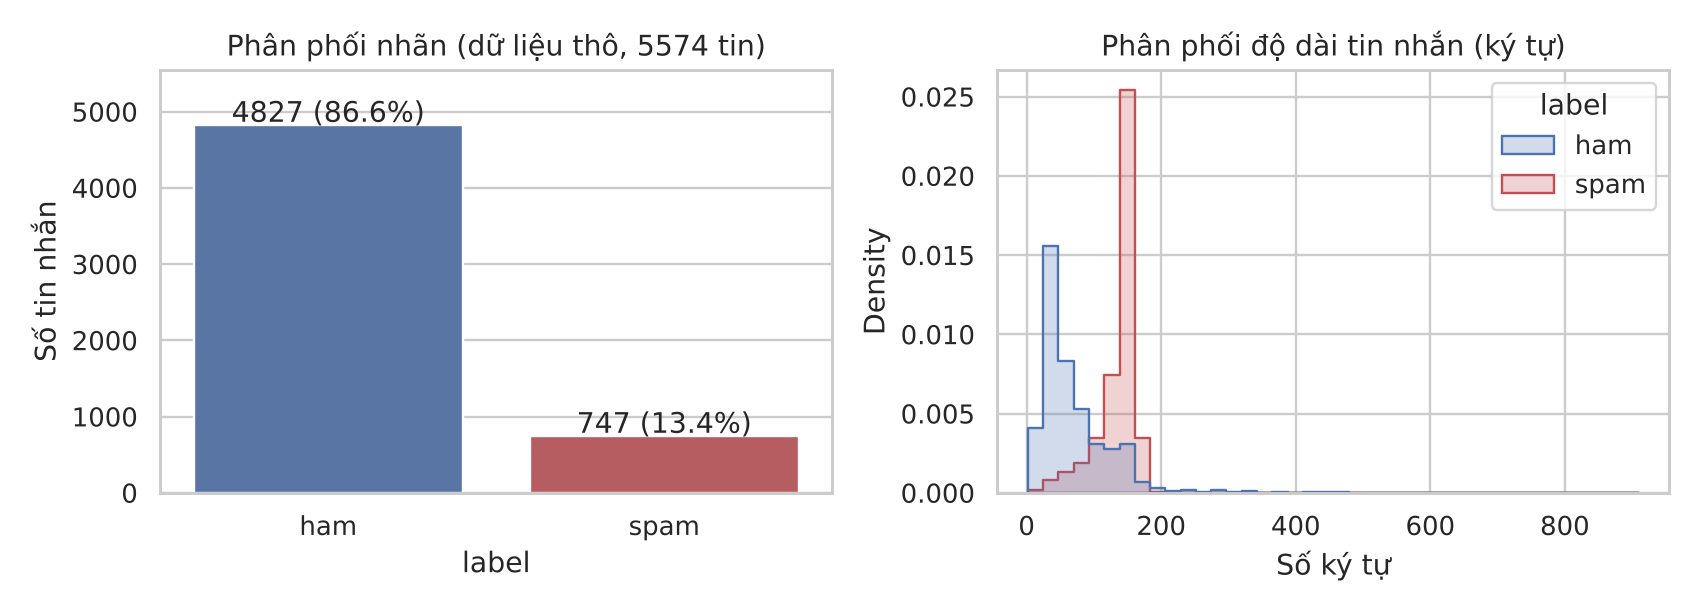
\includegraphics[width=\linewidth]{eda_label_length.png}
\caption{Phân phối nhãn (dữ liệu thô) và phân phối độ dài tin nhắn theo lớp.}\label{fig:eda1}
\end{figure}
\begin{figure}[H]\centering
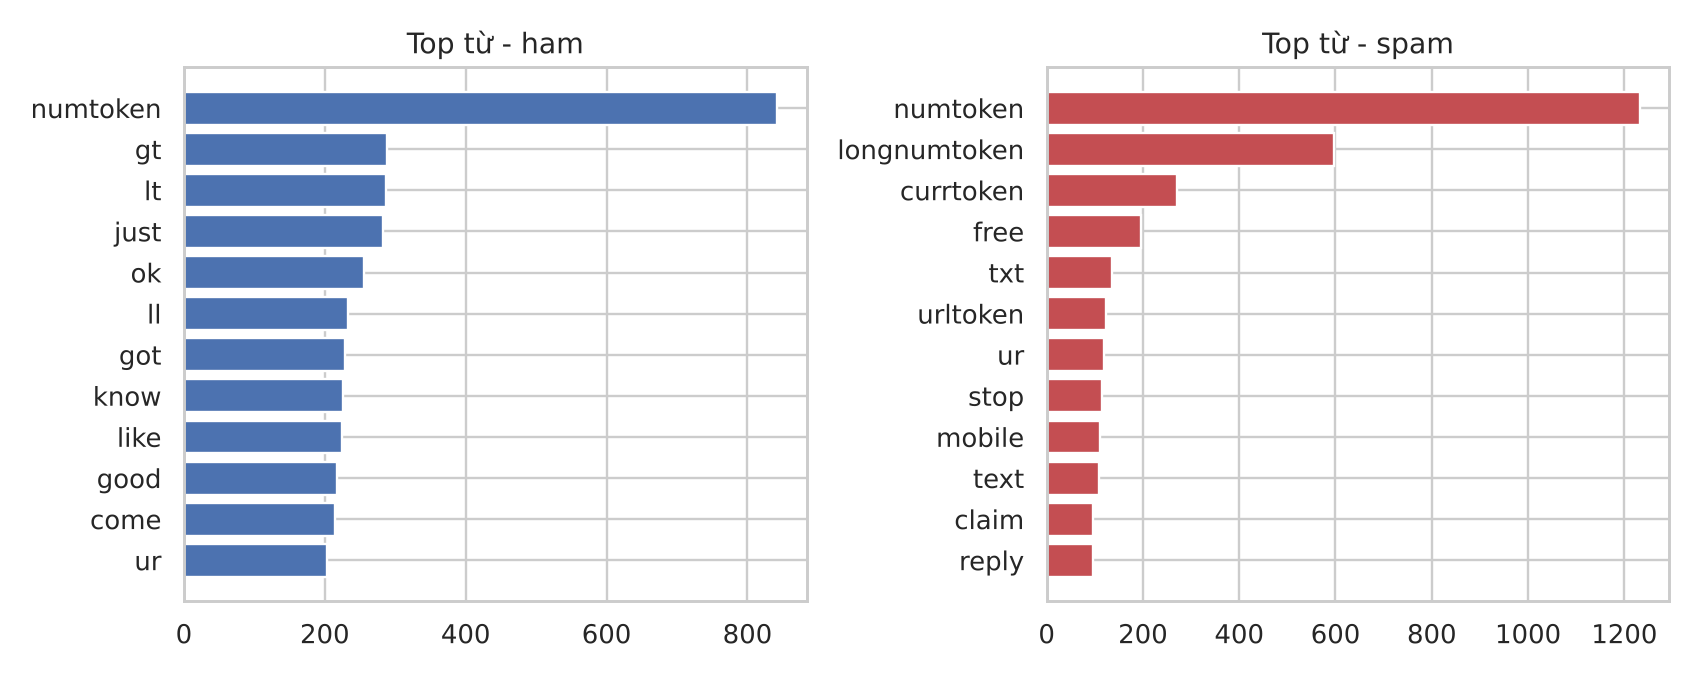
\includegraphics[width=0.95\linewidth]{eda_top_words.png}
\caption{Các từ phổ biến nhất của mỗi lớp (sau chuẩn hoá và bỏ stopword).}\label{fig:eda2}
\end{figure}

\paragraph{Giả thuyết hình thành từ EDA.}
\begin{enumerate}[nosep]
\item[H1.] Các chuỗi số dài, URL và ký hiệu tiền tệ là tín hiệu mạnh của \spam; mỗi số điện thoại cụ thể lại hiếm khi lặp lại, nên cần gom chúng về một token chung thay vì xoá bỏ.
\item[H2.] Từ khoá khuyến mãi (\texttt{free}, \texttt{claim}, \texttt{prize}, \texttt{win}, \texttt{txt}\ldots) giúp phân biệt; các từ này xuất hiện thành cụm nên bigram có thể hữu ích.
\item[H3.] Do mất cân bằng và chi phí lỗi khác nhau, cần ưu tiên F1/Precision/Recall của lớp \spam.
\end{enumerate}

% ====================================================================
\section{Thiết kế giải pháp và quy trình học máy}
\subsection{Sơ đồ pipeline}
\begin{figure}[H]\centering
\begin{tikzpicture}[node distance=0.5cm, every node/.style={font=\footnotesize},
 box/.style={draw,rounded corners,align=center,minimum height=1.0cm,minimum width=1.9cm,fill=blue!6},
 arr/.style={-{Stealth[length=2mm]}}]
\node[box] (a) {Dữ liệu thô\\5\,574 tin};
\node[box,right=of a] (b) {Bỏ trùng\\5\,171 tin};
\node[box,right=of b] (c) {Chia\\80/20\\(stratify)};
\node[box,right=of c,fill=orange!12] (d) {Tiền xử lý\\P0/P1/P2};
\node[box,right=of d,fill=orange!12] (e) {Biểu diễn\\BoW/TF-IDF};
\node[box,below=0.9cm of e,fill=green!10] (f) {Mô hình\\NB / K-NN / DT};
\node[box,left=of f,fill=green!10] (g) {GridSearchCV\\(5-fold, train)};
\node[box,left=of g,fill=purple!10] (h) {Đánh giá\\test};
\node[box,left=of h,fill=purple!10] (i) {Phân tích\\lỗi};
\draw[arr] (a)--(b); \draw[arr] (b)--(c); \draw[arr] (c)--(d); \draw[arr] (d)--(e);
\draw[arr] (e)--(f); \draw[arr] (f)--(g); \draw[arr] (g)--(h); \draw[arr] (h)--(i);
\begin{scope}[on background layer]
\node[draw,dashed,rounded corners,fit=(d)(e)(f),inner sep=3pt,label={[font=\scriptsize]above:\textit{Một sklearn Pipeline: fit chỉ trên dữ liệu huấn luyện}}] {};
\end{scope}
\end{tikzpicture}
\caption{Quy trình học máy của nhóm. Vector hoá và mô hình nằm trong cùng một Pipeline của scikit-learn.}\label{fig:pipe}
\end{figure}

\subsection{Chia dữ liệu và hạn chế rò rỉ dữ liệu}
\begin{itemize}[nosep]
\item Loại tin trùng \emph{trước} khi chia (xem mục EDA).
\item Chia hold-out 80/20 có phân tầng theo nhãn, \texttt{random\_state=42}: tập huấn luyện 4\,136 tin (522 \spam), tập kiểm thử 1\,035 tin (131 \spam).
\item Mọi lựa chọn (tiền xử lý, biểu diễn, siêu tham số) dùng \textbf{5-fold Stratified CV chỉ trên tập huấn luyện}; tập kiểm thử không tham gia việc chọn cấu hình.
\item Bộ vector hoá (từ vựng, IDF) nằm \emph{trong} \texttt{Pipeline}, nên được fit lại trên phần huấn luyện của từng fold, không nhìn thấy dữ liệu validation hay test.
\item Dữ liệu chỉ có văn bản và nhãn nên không có cột định danh hay cột rò rỉ nhãn.
\end{itemize}

\subsection{Tiền xử lý văn bản}
Nhóm so sánh ba mức, nhằm kiểm chứng giả thuyết H1:
\begin{itemize}[nosep]
\item \textbf{P0\_raw}: chỉ chuyển chữ thường và tách từ mặc định của vector hoá.
\item \textbf{P1\_normalize}: chữ thường; thay URL bằng \texttt{urltoken}, ký hiệu tiền tệ (£, \$, €) bằng \texttt{currtoken}, số từ 5 chữ số trở lên bằng \texttt{longnumtoken}, số còn lại bằng \texttt{numtoken}; bỏ ký tự đặc biệt. Cách này \emph{giữ tín hiệu} ``có số điện thoại/URL/tiền'' thay vì xoá bỏ.
\item \textbf{P2\_norm\_stop}: P1 cộng loại stopword tiếng Anh. Bước này có thể làm mất thông tin hữu ích (ví dụ ``to'', ``you'' xuất hiện khác nhau giữa hai lớp), nên được đưa vào thí nghiệm thay vì mặc định áp dụng.
\end{itemize}

\subsection{Biểu diễn đặc trưng}
Bốn cách biểu diễn: \textbf{BoW\_uni} (CountVectorizer, unigram), \textbf{TFIDF\_uni}, \textbf{BoW\_bi} (unigram + bigram, \texttt{min\_df=2}) và \textbf{TFIDF\_bi}. Kết hợp với ba mức tiền xử lý, mỗi mô hình có 12 cấu hình dữ liệu. Lưu ý: ở bốn cấu hình này bigram luôn đi kèm \texttt{min\_df=2} còn unigram dùng \texttt{min\_df=1}, nên hai yếu tố bị lẫn vào nhau; để tách riêng ảnh hưởng của n-gram, \texttt{min\_df}, \texttt{max\_df} và số đặc trưng, nhóm chạy thêm một thí nghiệm có kiểm soát (mục~\ref{sec:vec}).

\subsection{Thuật toán và siêu tham số}
\begin{itemize}[nosep]
\item \textbf{Multinomial Naive Bayes}: phù hợp với đặc trưng đếm/tần suất (Bài 4); giả định các từ độc lập có điều kiện theo lớp. Lưới: $\alpha\in\{0{,}001;\ 0{,}005;\ 0{,}01;\ 0{,}05;\ 0{,}1;\ 0{,}5;\ 1;\ 2\}$, \texttt{fit\_prior}$\in\{$True, False$\}$.
\item \textbf{K-NN}: phân loại theo biểu quyết của $k$ láng giềng gần nhất (Bài 3). Vì thuật toán dựa trên khoảng cách nên chọn metric là tham số quan trọng. Lưới: $k\in\{1,3,5,7,9,15\}$, metric $\in\{$cosine, euclidean$\}$, trọng số $\in\{$uniform, distance$\}$.
\item \textbf{Cây quyết định}: chia nút theo Gini hoặc Entropy (Bài 5). Lưới: \texttt{criterion}$\in\{$gini, entropy$\}$, \texttt{max\_depth}$\in\{$None, 5, 10, 20, 40$\}$, \texttt{min\_samples\_leaf}$\in\{1,2,5\}$. \texttt{random\_state=42}.
\end{itemize}

\subsection{Phương án baseline và quy trình chọn mô hình}
\textbf{Baseline} của nhóm là cách làm đơn giản nhất, hợp lý: BoW unigram, không tiền xử lý đặc biệt (P0), siêu tham số mặc định của scikit-learn cho cả ba mô hình. Mọi cải tiến được so với mốc này.

Quy trình gồm ba giai đoạn. (1) So sánh 36 cấu hình (3 mô hình $\times$ 3 tiền xử lý $\times$ 4 biểu diễn) với \emph{siêu tham số mặc định}. (2) Với Naive Bayes và K-NN, \emph{tinh chỉnh tham số cho từng ô} (tiền xử lý $\times$ biểu diễn) rồi mới chọn ô tốt nhất; với Cây quyết định (bất biến khi co giãn đặc trưng) chọn ô theo giai đoạn 1 rồi mới tinh chỉnh. Lý do thiết kế này được trình bày ở mục~\ref{sec:disc}: nếu chỉ so sánh với tham số mặc định, một số biểu diễn bị đánh giá thấp chỉ vì tham số chưa phù hợp. (3) Đánh giá trên tập kiểm thử một lần, kiểm tra độ ổn định qua 5 lần chia khác nhau và phân tích lỗi.

\subsection{Độ đo đánh giá}
Với lớp \spam{} là lớp dương: Accuracy, Precision $=\frac{TP}{TP+FP}$, Recall $=\frac{TP}{TP+FN}$, F1, ROC-AUC và ma trận nhầm lẫn (Bài 3). F1 của lớp \spam{} là tiêu chí chính để chọn cấu hình.

% ====================================================================
\section{Phân tích mã nguồn và chức năng}
Mã nguồn nằm trong repository với cấu trúc sau (hướng dẫn chạy trong \texttt{README.md}):
\begin{center}\small
\begin{tabular}{lp{10.5cm}}\toprule
\textbf{Tệp} & \textbf{Chức năng}\\\midrule
\texttt{src/common.py} & Nạp dữ liệu (UTF-8), hàm \texttt{normalize\_text}, từ điển cấu hình tiền xử lý và biểu diễn, hàm dựng \texttt{Pipeline}.\\
\texttt{src/run\_experiments.py} & Toàn bộ thí nghiệm: EDA, chia dữ liệu, so sánh 36 cấu hình, GridSearchCV, đánh giá test, ROC, độ ổn định theo seed, phân tích lỗi; ghi bảng vào \texttt{results/} và hình vào \texttt{figures/}.\\
\texttt{src/extra\_nb\_alpha\_check.py} & Kiểm tra độ nhạy của Naive Bayes với $\alpha$ lớn hơn.\\
\texttt{src/vectorizer\_sensitivity.py} & Thí nghiệm có kiểm soát về tham số vector hoá: n-gram, \texttt{min\_df}, \texttt{max\_df}, \texttt{max\_features}.\\
\texttt{src/predict.py} & Chương trình demo dòng lệnh dùng mô hình đã huấn luyện.\\
\texttt{src/demo\_app.py} & Ứng dụng demo web (Streamlit): nhập tin nhắn, xem nhãn SPAM/HAM, xác suất spam, so sánh ba mô hình và các từ ảnh hưởng (Naive Bayes).\\
\texttt{notebooks/sms\_spam\_pipeline.ipynb} & Notebook Jupyter chạy lại quy trình từng bước (EDA, baseline, so sánh, đánh giá, phân tích lỗi, demo), dùng chung hàm với \texttt{src/common.py}.\\
\texttt{report/make\_tables.py} & Sinh bảng LaTeX từ kết quả để số liệu báo cáo khớp với code.\\
\texttt{report/main.tex} & Báo cáo.\\\bottomrule
\end{tabular}
\end{center}

Hai đoạn mã then chốt. Đoạn thứ nhất là chuẩn hoá giữ tín hiệu (giả thuyết H1); đoạn thứ hai đặt vector hoá \emph{bên trong} Pipeline để tránh rò rỉ dữ liệu:
\begin{lstlisting}[language=Python]
def normalize_text(s):
    s = s.lower()
    s = URL_RE.sub(" urltoken ", s)
    s = CURR_RE.sub(" currtoken ", s)
    s = LONGNUM_RE.sub(" longnumtoken ", s)   # >= 5 chu so
    s = NUM_RE.sub(" numtoken ", s)
    s = re.sub(r"[^a-z\s]", " ", s)
    return re.sub(r"\s+", " ", s).strip()

Pipeline([("vec", make_vectorizer(prep, rep)), ("clf", model)])
\end{lstlisting}

% ====================================================================
\section{Thử nghiệm và kết quả}
\subsection{Thiết lập thí nghiệm}
Chia dữ liệu 80/20 phân tầng (\texttt{random\_state=42}); 5-fold Stratified CV (\texttt{shuffle=True}, \texttt{random\_state=42}) trên tập huấn luyện; tiêu chí chọn: F1 của lớp \spam; môi trường Python với scikit-learn (phiên bản trong \texttt{requirements.txt}). Baseline: BoW unigram, P0, tham số mặc định.

\subsection{Giai đoạn 1: tiền xử lý $\times$ biểu diễn với tham số mặc định}
Hình~\ref{fig:h1} cho F1 (CV) của 36 cấu hình. Tiền xử lý P1/P2 cải thiện rõ so với P0 ở Cây quyết định (BoW unigram tăng từ 0,834 lên 0,903 với P1 và 0,907 với P2) và cải thiện nhẹ ở Naive Bayes (0,936 lên 0,942 và 0,940). Với K-NN dùng khoảng cách Euclid mặc định, kết quả rất dao động và có cấu hình chỉ đạt F1 khoảng 0,4. Với Naive Bayes, các biểu diễn TF-IDF có F1 thấp hơn nhiều so với BoW khi dùng $\alpha=1$ (ví dụ 0,751 với P0 + TF-IDF unigram); phần thảo luận giải thích đây chủ yếu là hiệu ứng của tham số mặc định chứ không phải của TF-IDF.

\begin{figure}[H]\centering
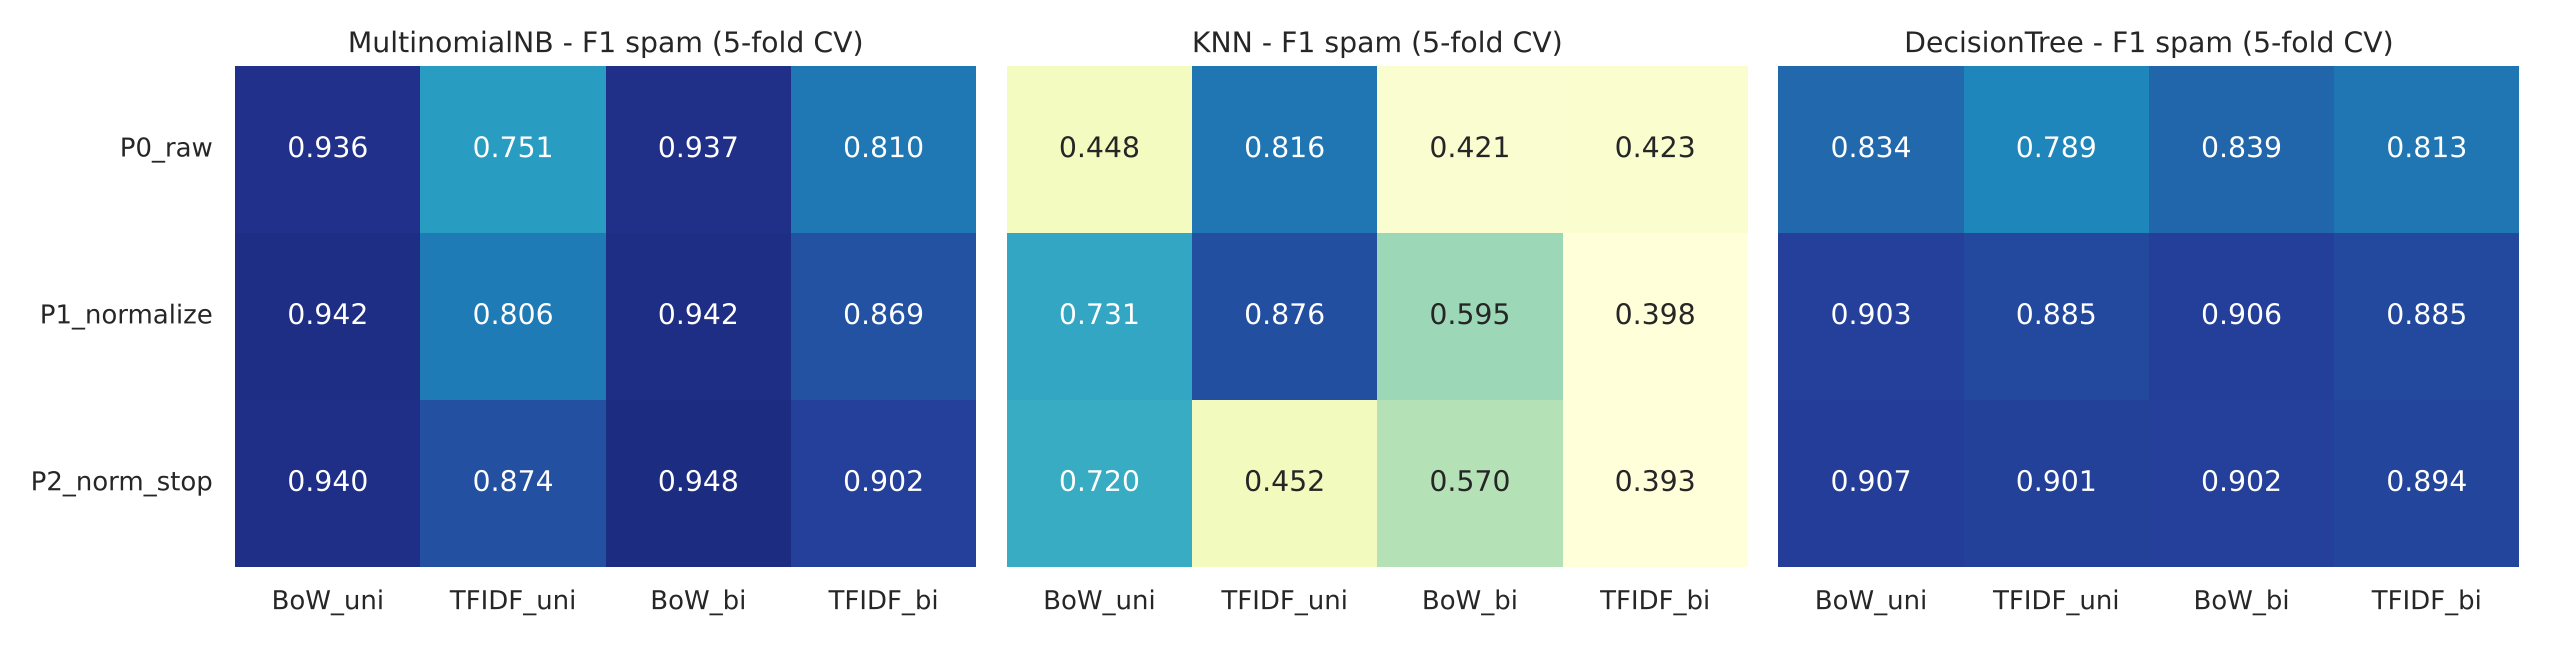
\includegraphics[width=\linewidth]{stage1_heatmap_cv_f1.png}
\caption{F1 của lớp \spam{} (5-fold CV, tập train) cho 36 cấu hình với siêu tham số mặc định.}\label{fig:h1}
\end{figure}

\subsection{Giai đoạn 2: tinh chỉnh tham số theo từng cấu hình}
Hình~\ref{fig:h2} cho thấy khi mỗi ô được tinh chỉnh tham số, khoảng cách giữa các biểu diễn thu hẹp mạnh: với Naive Bayes, F1 (CV) của mọi ô nằm trong khoảng 0,935--0,952, và TF-IDF không còn thua BoW một cách hệ thống. K-NN đều chọn khoảng cách cosine, trọng số \texttt{distance}, và tốt nhất với TF-IDF unigram sau chuẩn hoá (F1 CV 0,918, so với 0,876 khi dùng tham số mặc định).

\begin{figure}[H]\centering
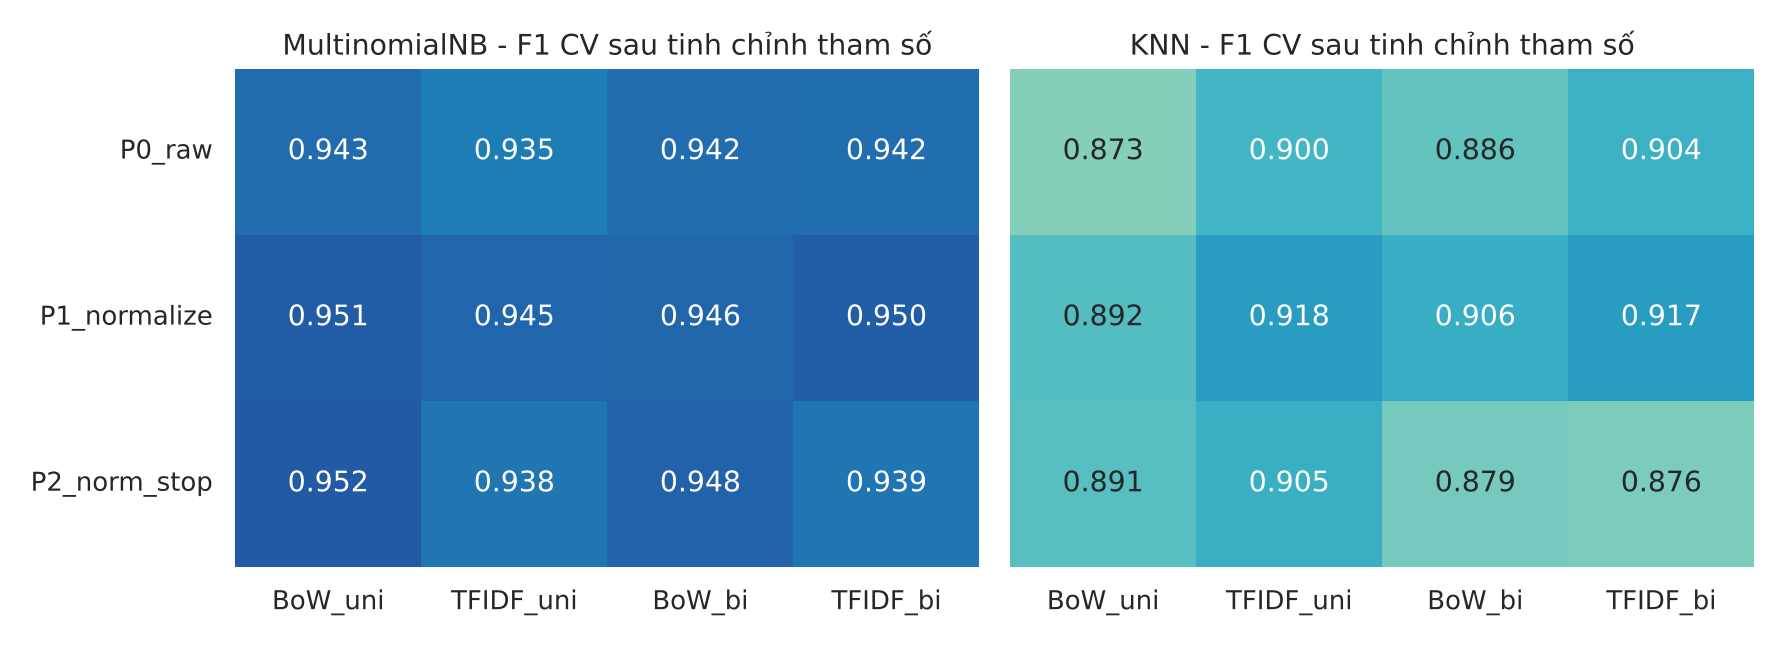
\includegraphics[width=0.85\linewidth]{stage2_heatmap_tuned_cv_f1.png}
\caption{F1 CV sau khi tinh chỉnh tham số trong từng ô, cho Naive Bayes và K-NN.}\label{fig:h2}
\end{figure}

\TabCfg

Hình~\ref{fig:curves} cho thấy ảnh hưởng của các tham số chính trong cấu hình đã chọn. Với Naive Bayes, F1 đạt đỉnh tại $\alpha=2$. Vì đỉnh này nằm ở giá trị lớn nhất của lưới, nhóm chạy thêm kiểm tra với $\alpha$ lên đến 10 (Bảng~\ref{tab:alpha}): đỉnh vẫn ở $\alpha=2$ và ổn định qua ba cách chia fold; tăng $\alpha$ hơn nữa làm Precision tăng nhưng Recall giảm. Với K-NN, $k$ từ 7 trở lên cho kết quả gần như phẳng, và cosine vượt trội Euclid ở mọi $k$. Với Cây quyết định, độ sâu 10 cho F1 CV cao nhất, và tăng thêm độ sâu không cải thiện.

\begin{figure}[H]\centering
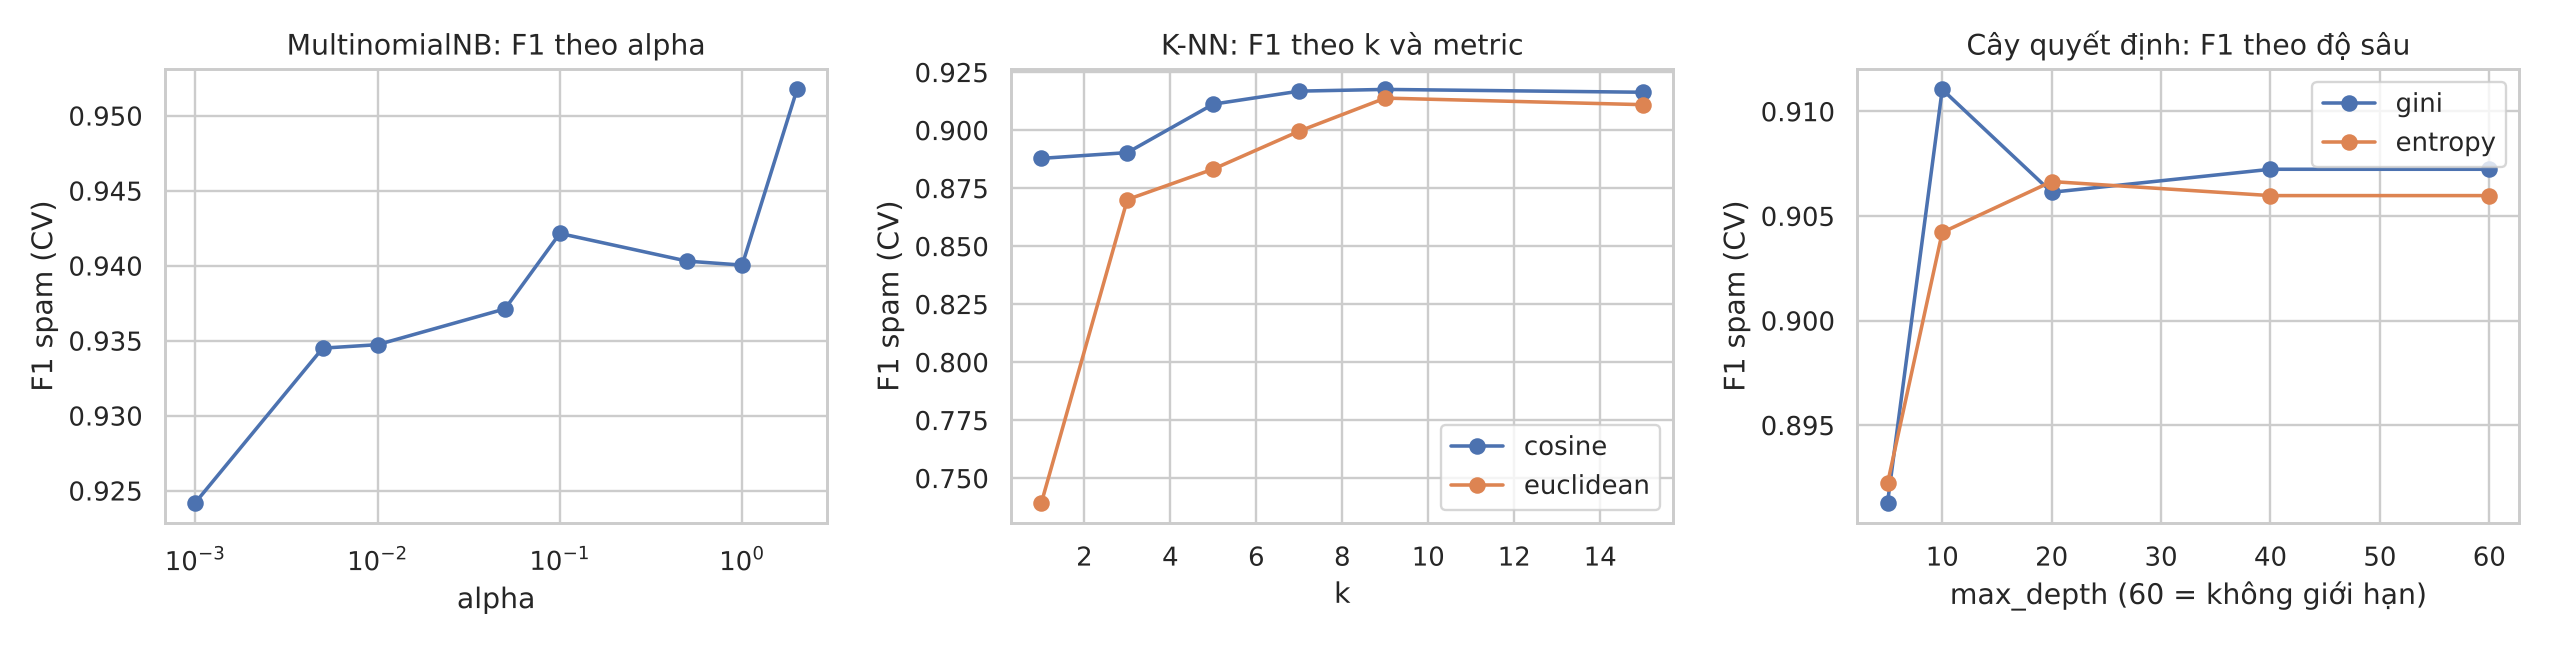
\includegraphics[width=\linewidth]{stage2_param_curves.png}
\caption{F1 (CV) theo siêu tham số quan trọng của từng mô hình.}\label{fig:curves}
\end{figure}

\TabAlpha

\subsection{Ảnh hưởng của tham số vector hoá}\label{sec:vec}
Hướng dẫn yêu cầu so sánh n-gram, \texttt{min\_df}, \texttt{max\_df} hoặc số đặc trưng. Với mỗi mô hình, nhóm giữ nguyên tiền xử lý, loại biểu diễn và siêu tham số đã chọn, rồi đổi \emph{từng} tham số vector hoá (5-fold CV chỉ trên tập train, không dùng tập test). Kết quả ở Bảng~\ref{tab:vecgrid}, Bảng~\ref{tab:vecfeat} và Hình~\ref{fig:vec}.

\TabVecGrid
\TabVecFeat

\begin{figure}[H]\centering
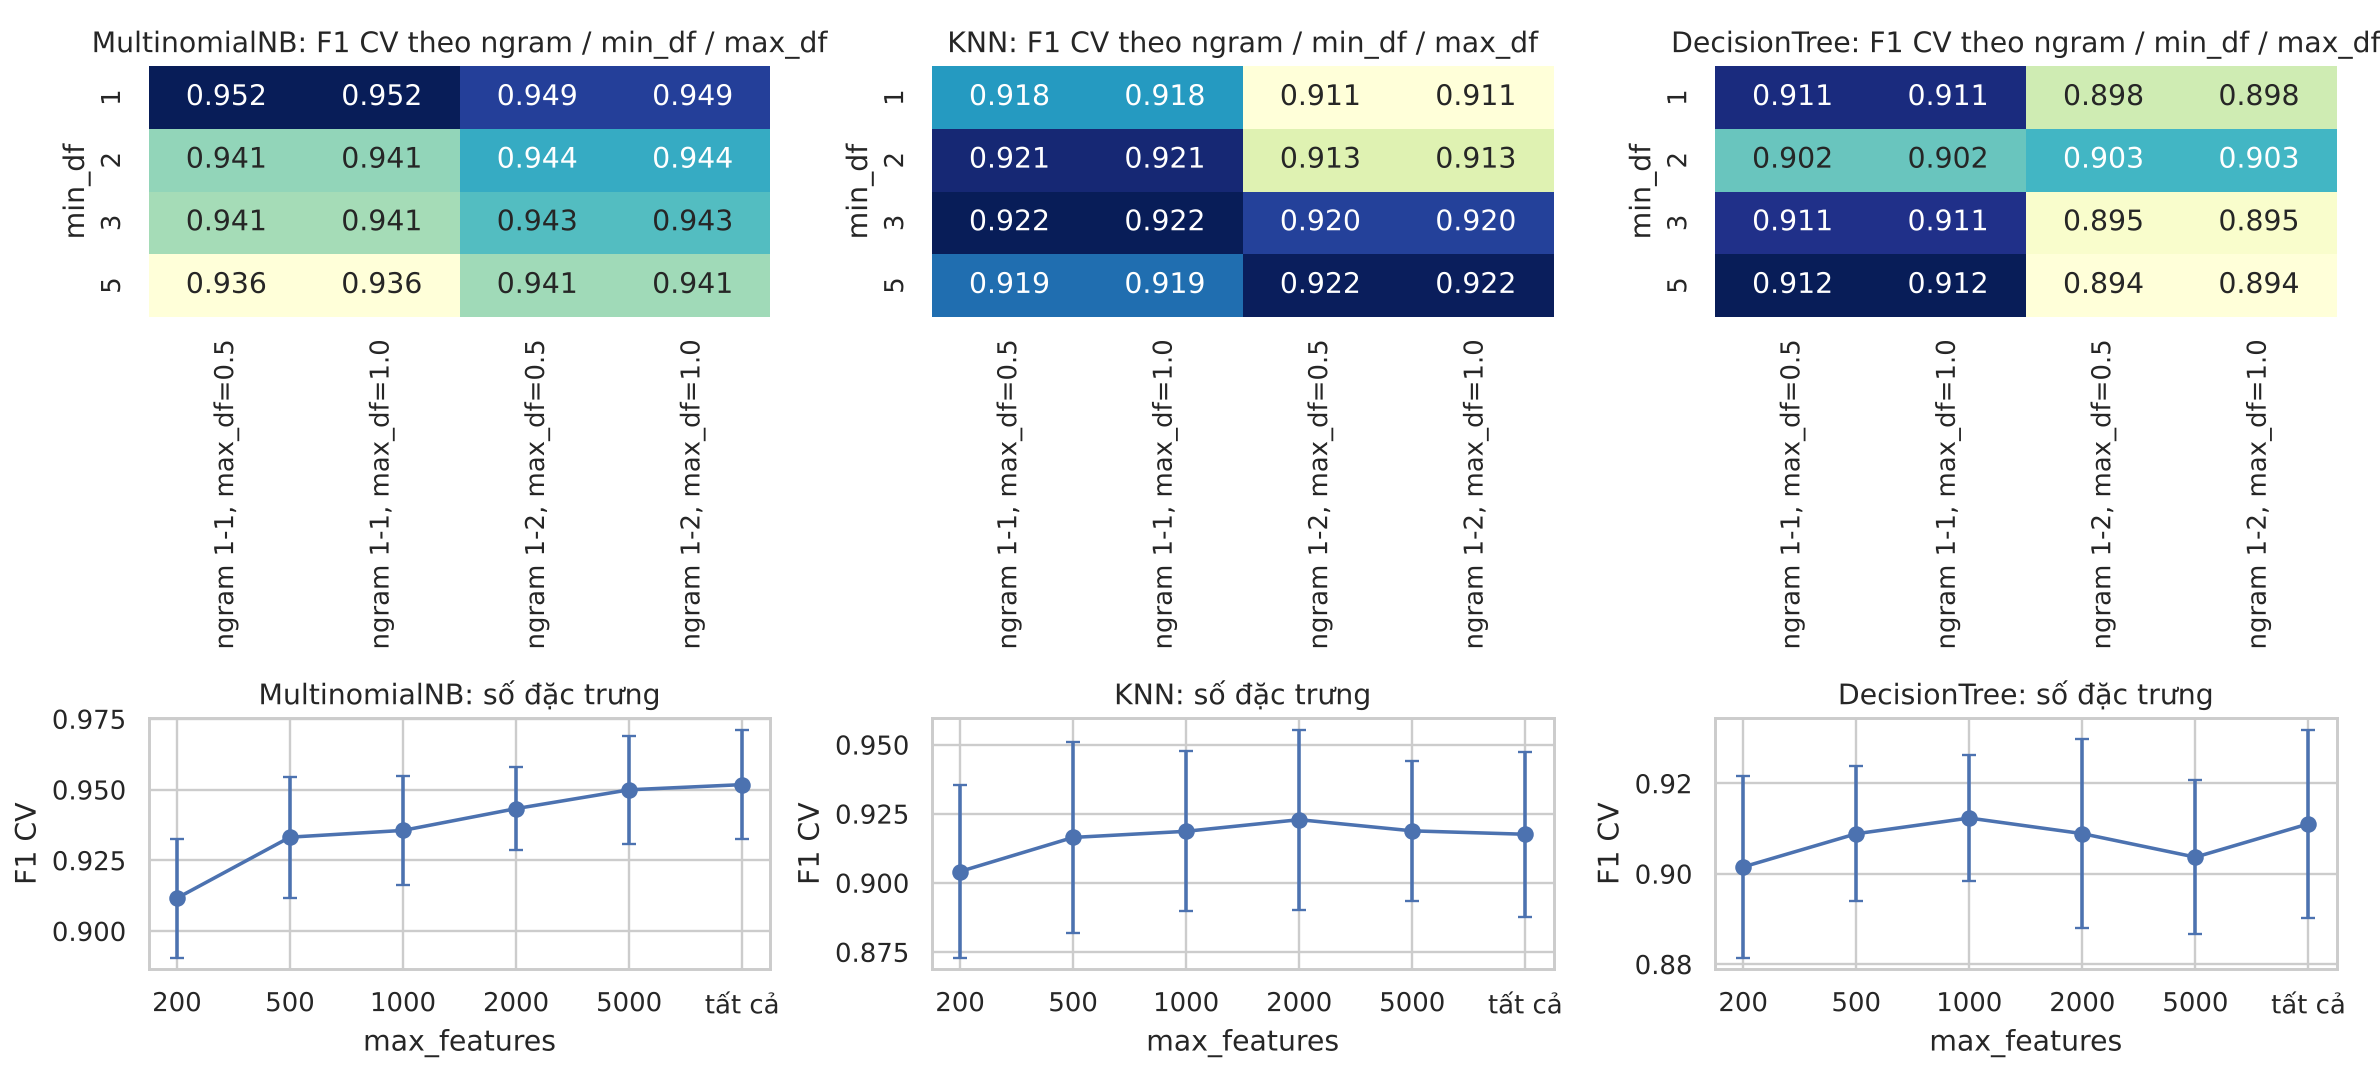
\includegraphics[width=\linewidth]{vectorizer_sensitivity.png}
\caption{F1 CV theo n-gram, \texttt{min\_df}, \texttt{max\_df} (hàng trên) và theo số đặc trưng (hàng dưới, thanh sai số là độ lệch chuẩn giữa các fold).}\label{fig:vec}
\end{figure}

Các quan sát chính: (i) \texttt{max\_df}=0,5 và 1,0 cho kết quả giống hệt nhau ở cả ba mô hình, nghĩa là không từ nào xuất hiện trong hơn một nửa số tin nên tham số này không có tác dụng ở bài toán này; (ii) toàn bộ lưới n-gram $\times$ \texttt{min\_df} chỉ dao động trong khoảng 0,936--0,952 (Naive Bayes), 0,911--0,922 (K-NN) và 0,894--0,913 (Cây quyết định), trong khi độ lệch chuẩn F1 giữa các fold là khoảng 0,017, 0,026 và 0,019, nên các khác biệt này nằm trong mức nhiễu; (iii) khi so sánh công bằng ở cùng \texttt{min\_df}, bigram không tạo cải thiện đáng kể (Naive Bayes với \texttt{min\_df}=2: 0,941 so với 0,944); (iv) chỉ khi cắt từ vựng xuống còn khoảng 200 từ, F1 mới giảm rõ (Naive Bayes từ 0,952 xuống 0,912, gấp khoảng hai lần độ lệch chuẩn), còn từ 2\,000 từ trở lên kết quả gần như bằng dùng toàn bộ từ vựng.

\subsection{Kết quả trên tập kiểm thử}
Bảng~\ref{tab:basetuned} so sánh baseline với cấu hình tinh chỉnh; Bảng~\ref{tab:final} là kết quả cuối cùng với số lỗi tuyệt đối.

\TabBaseTuned
\TabFinal

\begin{figure}[H]\centering
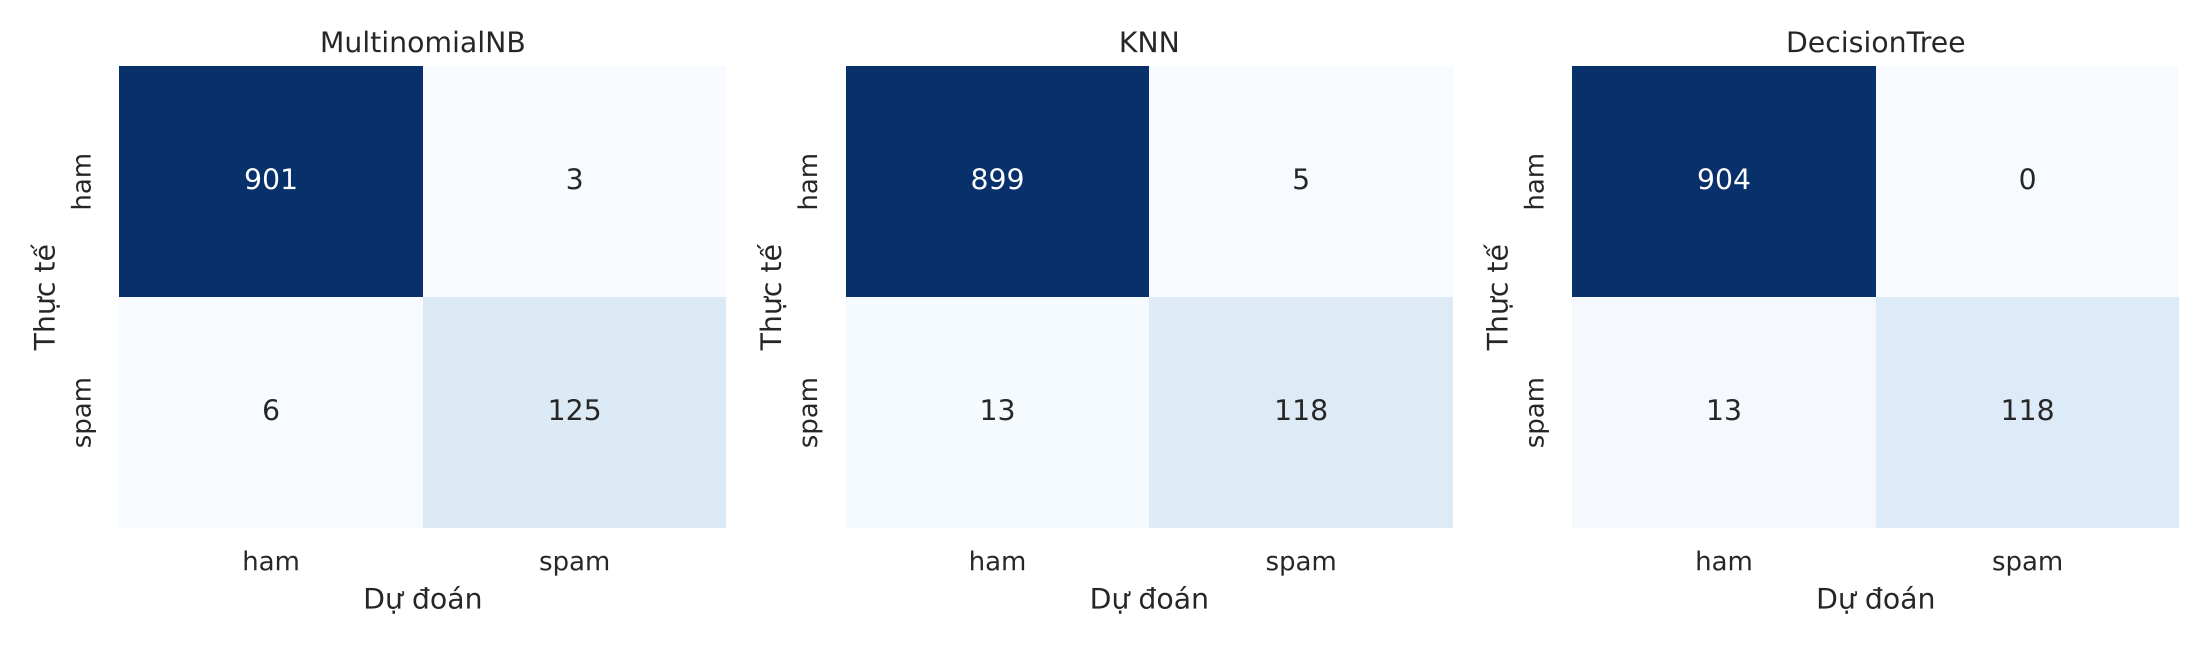
\includegraphics[width=\linewidth]{confusion_matrices.png}
\caption{Ma trận nhầm lẫn trên tập kiểm thử (lớp dương: \spam).}\label{fig:cm}
\end{figure}

\begin{figure}[H]\centering
\begin{subfigure}{0.48\linewidth}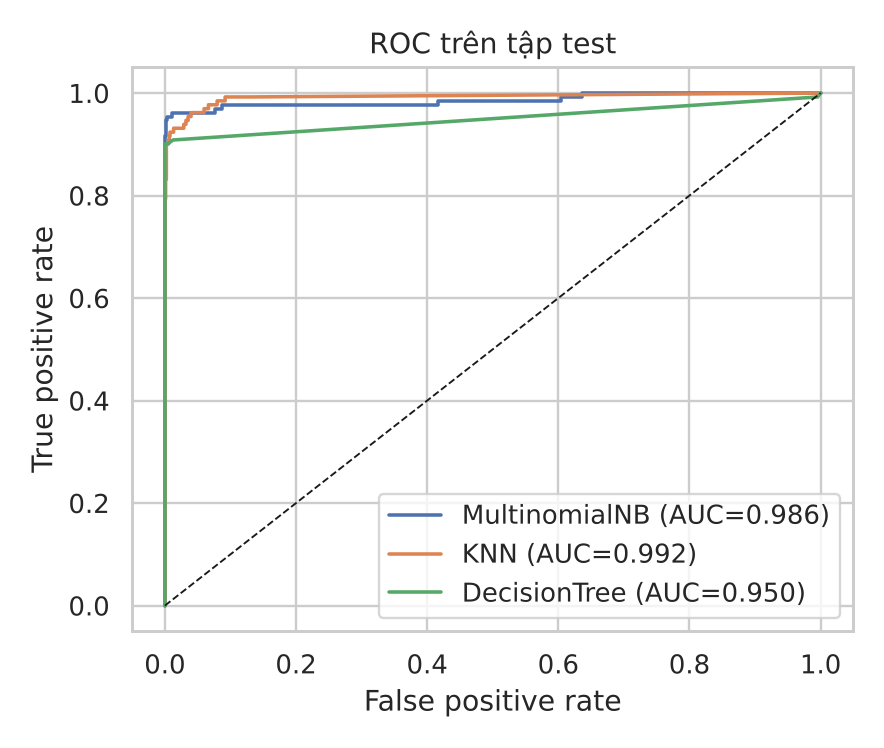
\includegraphics[width=\linewidth]{roc_curves.png}\caption{ROC}\end{subfigure}
\begin{subfigure}{0.50\linewidth}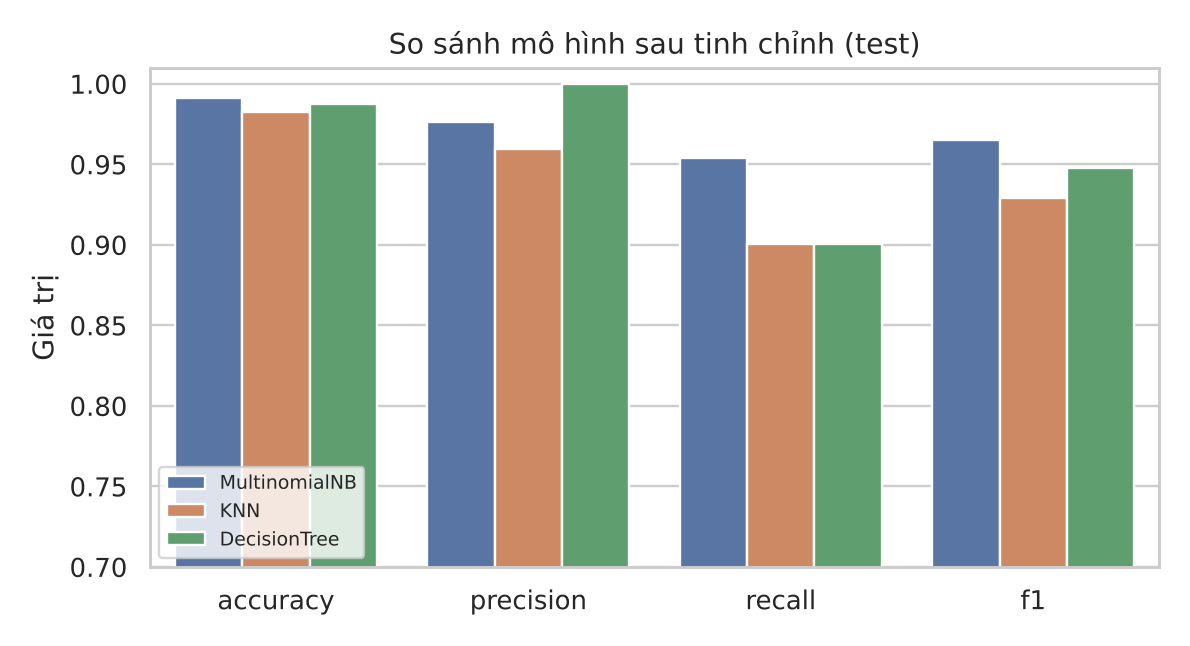
\includegraphics[width=\linewidth]{final_metric_bars.png}\caption{Các độ đo}\end{subfigure}
\caption{Đường ROC và so sánh các độ đo của ba mô hình sau tinh chỉnh.}\label{fig:roc}
\end{figure}

Một lần chia duy nhất với 131 tin \spam{} cho kết quả nhạy với vài tin nhắn, vì sai khác 1 tin \spam{} đã đổi Recall khoảng 0,8 điểm phần trăm. Nhóm do đó lặp lại với 5 cách chia khác nhau (Bảng~\ref{tab:seeds}).

\TabSeeds

Về chi phí tính toán, dự đoán 1\,035 tin mất khoảng 0,04 giây với Naive Bayes và Cây quyết định, và khoảng 0,12 giây với K-NN (K-NN phải lưu toàn bộ tập huấn luyện và tính khoảng cách khi dự đoán). Thời gian đo trên một máy một lõi nên chỉ mang tính tham khảo.

\subsection{Ứng dụng demo}
Nhóm xây dựng ứng dụng web nhỏ bằng Streamlit (\texttt{streamlit run src/demo\_app.py}) sử dụng đúng các cấu hình đã chọn ở Bảng~\ref{tab:cfg}. Người dùng nhập một tin nhắn tiếng Anh hoặc chọn tin mẫu; ứng dụng trả về nhãn \spam/\ham, xác suất spam của mô hình được chọn, bảng so sánh dự đoán của cả ba mô hình, và phần giải thích gồm tin nhắn sau chuẩn hoá cùng các từ đẩy dự đoán về phía spam hay ham (với Naive Bayes). Ứng dụng chỉ dùng cho mục đích minh hoạ: mô hình được huấn luyện trên dữ liệu tiếng Anh cũ nên không nên dùng để lọc tin nhắn thật.

% ====================================================================
\section{Thảo luận và so sánh}\label{sec:disc}
\subsection{Ảnh hưởng của tiền xử lý và biểu diễn}
\paragraph{Tiền xử lý giữ tín hiệu có tác dụng rõ rệt.} Chuyển từ P0 sang P1 cải thiện F1 CV của Cây quyết định từ 0,834 lên 0,903 và của Naive Bayes (BoW unigram, tham số mặc định) từ 0,936 lên 0,942. Cây quyết định hưởng lợi nhiều nhất: token \texttt{longnumtoken} chiếm độ quan trọng 0,746 trong cây cuối cùng. Giải thích hợp lý (phù hợp với H1) là mỗi số điện thoại cụ thể gần như chỉ xuất hiện một lần nên ở P0 chúng thành các đặc trưng hiếm vô dụng; sau khi gom về một token chung, sự kiện ``tin có số dài'' (76,7\% spam so với 0,1\% ham) trở thành đặc trưng mạnh. Các đặc trưng quan trọng nhất của cây là \DTtop.

\paragraph{Loại stopword cho hiệu quả nhỏ.} Giữa P1 và P2, F1 CV của Naive Bayes sau tinh chỉnh chỉ khác nhau trong khoảng 0,01 và theo cả hai hướng tuỳ biểu diễn; với K-NN, P2 thường kém hơn P1. Nhóm kết luận stopword không phải yếu tố quyết định ở bài toán này, và chênh lệch giữa các ô tốt nhất của Naive Bayes nằm trong mức nhiễu của CV (độ lệch chuẩn F1 giữa các fold ở giai đoạn 1 của Naive Bayes khoảng 0,016--0,041), nên việc ô P2 + BoW unigram được chọn không nên bị diễn giải là bằng chứng rằng nó vượt trội thật sự.

\paragraph{TF-IDF ``thua'' BoW chỉ do tham số mặc định.} Với $\alpha=1$, Naive Bayes trên TF-IDF cho F1 CV thấp (0,751--0,902) trong khi BoW đạt 0,936--0,948. Sau khi tinh chỉnh, các ô TF-IDF đạt 0,935--0,950 và các $\alpha$ tốt nhất của chúng nhỏ hơn đáng kể (0,005--0,1). Điều này phù hợp với giả thuyết rằng giá trị TF-IDF (chuẩn hoá L2, rất nhỏ) khiến hệ số làm trơn $\alpha=1$ chiếm ưu thế so với tần suất thực tế và làm xác suất theo lớp bị san phẳng; nhóm chưa kiểm chứng trực tiếp cơ chế này. Bài học phương pháp: so sánh các biểu diễn với tham số cố định dễ dẫn tới kết luận sai, nên nhóm tinh chỉnh tham số theo từng biểu diễn trước khi so sánh.

\paragraph{Bigram, \texttt{min\_df} và \texttt{max\_df}.} Thí nghiệm có kiểm soát ở mục~\ref{sec:vec} cho thấy bigram không mang lại cải thiện nhất quán khi so ở cùng \texttt{min\_df}, và các khác biệt nằm trong mức nhiễu của CV. Giả thuyết H2 về lợi ích của bigram do đó \emph{không được ủng hộ} trong thí nghiệm này; một giải thích có thể là tin nhắn ngắn nên các cụm hai từ hiếm khi lặp lại đủ nhiều để mô hình học được (nhóm chưa kiểm chứng trực tiếp). \texttt{max\_df} không có tác dụng, và việc giảm số đặc trưng chỉ gây hại khi cắt rất mạnh (xuống khoảng 200 từ), nên có thể giữ toàn bộ từ vựng.

\subsection{So sánh ba thuật toán}
\begin{itemize}[nosep]
\item \textbf{Naive Bayes} đạt kết quả tốt nhất trên tập kiểm thử (F1 0,965; chỉ 9 lỗi: 3 FP, 6 FN) và cũng cao nhất khi lặp qua 5 cách chia (F1 $0{,}947\pm0{,}020$). Ưu điểm: Recall cao và ổn định, huấn luyện và dự đoán nhanh, các từ có trọng số lớn dễ diễn giải. Nhược điểm: giả định độc lập có điều kiện giữa các từ, và rất nhạy với $\alpha$ (Bảng~\ref{tab:alpha}).
\item \textbf{K-NN} (cosine, TF-IDF) có ROC-AUC cao nhất (0,992) nhưng F1 trên test chỉ 0,929 do Recall 0,901: thứ tự xếp hạng tốt nhưng ngưỡng quyết định (biểu quyết $k=9$ có trọng số) chưa tối ưu cho lớp thiểu số. Phải chọn đúng metric: baseline Euclid trên vector đếm chỉ đạt F1 0,422, tức là bỏ sót 73\% spam, vì khoảng cách Euclid bị chi phối bởi độ dài tin nhắn, đúng như vấn đề ``khoảng cách có công bằng không'' ở Bài 3.
\item \textbf{Cây quyết định} đạt Precision 1,000 trên test (không chặn nhầm tin nào) nhưng Recall chỉ 0,901. Qua 5 lần chia, F1 trung bình thấp nhất ($0{,}907\pm0{,}018$) và Recall chỉ $0{,}860$; kết quả test 0,948 ở \texttt{random\_state=42} nằm ở phía thuận lợi của phân bố này. Cây chủ yếu dựa vào vài luật cứng (có số dài, có URL, từ khoá), nên bắt tốt spam điển hình nhưng bỏ sót spam không có các dấu hiệu đó.
\end{itemize}

Về mức độ chắc chắn của kết luận: chênh lệch giữa Naive Bayes và Cây quyết định ($0{,}947$ so với $0{,}907$) lớn hơn nhiều độ lệch chuẩn nên khá đáng tin, còn chênh lệch giữa Naive Bayes và K-NN ($0{,}947$ so với $0{,}934$) nhỏ hơn độ lệch chuẩn nên \emph{không đủ để khẳng định} mô hình nào tốt hơn. Nhóm không chạy kiểm định thống kê chính thức.

\subsection{Phân tích lỗi}
Trên tập kiểm thử, Naive Bayes sai 9 tin, K-NN 18, Cây quyết định 13; có \textbf{5 tin bị cả ba mô hình cùng phân loại sai}, tức là lỗi phần lớn do tính chất dữ liệu chứ không riêng một thuật toán.

\paragraph{Dương tính giả (3 tin ham bị chặn nhầm).} Cả ba tin đều ngắn (trung bình khoảng 31 ký tự) và chứa từ thương mại: \emph{``Nokia phone is lovly..''}, \emph{``Have you laid your airtel line to rest?''}, \emph{``Unlimited texts. Limited minutes.''}. Trong từ vựng 6\,516 từ của mô hình Naive Bayes, \texttt{nokia} xếp hạng 4 về trọng số spam (log-odds), \texttt{line} xếp hạng 90 và \texttt{unlimited} xếp hạng 148; còn \texttt{lovly} không có trong từ vựng. Tin quá ngắn nên không có thêm bằng chứng nào để bù lại các từ nghiêng về spam này. Nhóm từ spam mạnh nhất là: \NBtopspam. Đây là loại lỗi đáng chú ý vì chi phí cao hơn trong ứng dụng thực tế.

\paragraph{Âm tính giả (6 tin spam bị bỏ sót).} Chỉ 1/6 tin có chuỗi số dài, và không tin nào có URL hay ký hiệu tiền tệ, trong khi ở nhóm spam bắt đúng các tỉ lệ này lần lượt là 84\%, 12\% và 30\%. Các tin bị bỏ sót gồm quảng cáo người lớn không nêu số (``Would you like to see my XXX pics\ldots''), tin kiểu đố vui có từ khoá ít điển hình (câu hỏi về phim Simpsons, ``Send A, B or C'') và một tin quảng bá sự kiện có văn phong gần với tin cá nhân (``Xmas \& New Years Eve tickets are now on sale\ldots''). Giả thuyết của nhóm: mô hình dựa mạnh vào các dấu hiệu cấu trúc, nên spam ``giống tin thường'' sẽ là điểm yếu chung của cả ba thuật toán.

\subsection{Hạn chế}
\begin{itemize}[nosep]
\item \textbf{Cỡ mẫu kiểm thử nhỏ}: 131 tin \spam, nên Recall chênh nhau $\sim$0,8 điểm phần trăm cho mỗi tin; các khoảng chênh lệch dưới $\sim$0,02 giữa mô hình không đáng tin. Nhóm chưa tính khoảng tin cậy bootstrap.
\item \textbf{Artefact của dữ liệu}: 197 tin \ham{} chứa chuỗi \texttt{\&lt;\#\&gt;} (mã HTML của số đã bị ẩn danh), còn không tin \spam{} nào có; sau chuẩn hoá nó thành token \texttt{lt}, \texttt{gt} và xuất hiện trong nhóm từ ham mạnh nhất của Naive Bayes (\NBtopham). Mô hình có thể đang khai thác dấu hiệu phụ thuộc cách xây dựng dữ liệu này, không có giá trị trên tin nhắn thật.
\item \textbf{Gần trùng lặp}: ta chỉ loại tin trùng \emph{hoàn toàn}; các tin spam cùng một chiến dịch với vài chữ khác nhau vẫn có thể nằm ở cả train và test, khiến kết quả lạc quan.
\item \textbf{Phân phối dữ liệu}: dữ liệu cũ, chủ yếu tiếng Anh Anh/Singapore; mô hình chưa được kiểm tra trên spam hiện đại hay ngôn ngữ khác.
\item \textbf{Tập tìm kiếm tham số có giới hạn}; F1 CV cao nhất trong nhiều cấu hình có thể hơi lạc quan do chọn max trên nhiều ô.
\end{itemize}

% ====================================================================
\section{Tổng kết và hướng phát triển}
\subsection{Kết quả chính}
Nhóm đã xây dựng quy trình hoàn chỉnh cho phân loại tin nhắn rác: loại bản trùng, chia dữ liệu có phân tầng, so sánh 12 cấu hình dữ liệu cho mỗi trong ba thuật toán, tinh chỉnh tham số bằng CV trên tập huấn luyện và đánh giá bằng nhiều độ đo. Các kết luận chính:
\begin{enumerate}[nosep]
\item Cả ba mô hình đều đạt Accuracy trên 98\% trên test, nhưng do dữ liệu mất cân bằng nên Accuracy ít phân biệt; F1 của lớp \spam{} cho thấy rõ khác biệt hơn.
\item Chuẩn hoá giữ tín hiệu (gom số dài, URL, tiền tệ thành token) là cải tiến tiền xử lý hiệu quả nhất, đặc biệt với Cây quyết định.
\item Naive Bayes ($\alpha=2$, BoW unigram, P2) cho F1 test 0,965 và trung bình 0,947 qua 5 lần chia, là lựa chọn tốt nhất trong ba mô hình, dù sự khác biệt với K-NN chưa đủ vững để khẳng định chắc chắn.
\item So sánh biểu diễn với siêu tham số mặc định có thể dẫn tới kết luận sai (TF-IDF, K-NN Euclid), nên cần tinh chỉnh tham số theo từng biểu diễn trước khi so sánh.
\end{enumerate}

\subsection{Hướng phát triển}
\begin{itemize}[nosep]
\item Điều chỉnh \emph{ngưỡng quyết định} theo chi phí lỗi (ví dụ ưu tiên Precision) và đánh giá bằng đường Precision--Recall.
\item Tính khoảng tin cậy bootstrap, chia dữ liệu theo nhóm để tránh gần trùng lặp, và đánh giá trên dữ liệu spam mới hơn.
\item Thử biểu diễn nâng cao (n-gram ký tự, embedding câu) và thêm đặc trưng thủ công (độ dài, tỉ lệ chữ hoa) như phần mở rộng.
\item Triển khai ứng dụng demo lên máy chủ hoặc đám mây, và bổ sung cơ chế cho người dùng báo lại tin bị phân loại sai.
\end{itemize}

% ====================================================================
\appendix
\section{Khai báo sử dụng công cụ AI}
\textbf{[Nhóm điền và chỉnh sửa phần này cho đúng thực tế.]} Nhóm đã sử dụng trợ lý AI (Claude, Anthropic) để hỗ trợ: (i) gợi ý cấu trúc pipeline và viết bản đầu của mã nguồn; (ii) chạy thí nghiệm và sinh bảng, hình; (iii) soạn bản nháp báo cáo. Nhóm chịu trách nhiệm về tính đúng đắn của nội dung: các thành viên đã đọc, chạy lại mã nguồn, kiểm tra số liệu và có thể giải thích pipeline cũng như kết quả khi bảo vệ. Chi tiết trong tệp \texttt{AI\_USAGE.md} của repository.

\section{Tài liệu tham khảo}
\begin{enumerate}[nosep]
\item Almeida, T.A., Gómez Hidalgo, J.M., Yamakami, A. \emph{Contributions to the study of SMS Spam Filtering: New Collection and Results}. ACM Symposium on Document Engineering, 2011. Dữ liệu: Almeida, T., Hidalgo, J. (2011). \emph{SMS Spam Collection}. UCI Machine Learning Repository, \url{https://doi.org/10.24432/C5CC84}, giấy phép CC BY 4.0.
\item Müller, A.C., Guido, S. \emph{Introduction to Machine Learning with Python}. O'Reilly.
\item Vũ Hữu Tiệp. \emph{Machine Learning cơ bản}.
\item Bài giảng học phần Nhập môn Học máy (Bài 2--6), ThS. Lê Thị Thùy Trang, Đại học Đại Nam.
\end{enumerate}

\end{document}
